% !TEX encoding = UTF-8 Unicode
\documentclass[a4paper]{article}

\usepackage{color}
\usepackage{url}
\usepackage[T2A]{fontenc} % enable Cyrillic fonts
\usepackage[utf8]{inputenc} % make weird characters work
\usepackage{graphicx}
\graphicspath{ {./images/} }
\usepackage{amsfonts}
\usepackage[english,serbian]{babel}
\usepackage{subcaption}
%\usepackage[english,serbianc]{babel} %ukljuciti babel sa ovim opcijama, umesto gornjim, ukoliko se koristi cirilica

\usepackage[unicode]{hyperref}
\hypersetup{colorlinks,citecolor=green,filecolor=green,linkcolor=blue,urlcolor=blue}

\usepackage{listings}
\usepackage{mathtools}
\usepackage{dirtytalk}
\usepackage{epigraph}
\usepackage{amssymb}


%\newtheorem{primer}{Пример}[section] %ćirilični primer
\newtheorem{primer}{Primer}[section]

\definecolor{mygreen}{rgb}{0,0.6,0}
\definecolor{mygray}{rgb}{0.5,0.5,0.5}
\definecolor{mymauve}{rgb}{0.58,0,0.82}

\lstset{ 
  backgroundcolor=\color{white},   % choose the background color; you must add \usepackage{color} or \usepackage{xcolor}; should come as last argument
  basicstyle=\scriptsize\ttfamily,        % the size of the fonts that are used for the code
  breakatwhitespace=false,         % sets if automatic breaks should only happen at whitespace
  breaklines=true,                 % sets automatic line breaking
  captionpos=b,                    % sets the caption-position to bottom
  commentstyle=\color{mygreen},    % comment style
  deletekeywords={...},            % if you want to delete keywords from the given language
  escapeinside={\%*}{*)},          % if you want to add LaTeX within your code
  extendedchars=true,              % lets you use non-ASCII characters; for 8-bits encodings only, does not work with UTF-8
  firstnumber=1000,                % start line enumeration with line 1000
  frame=single,	                   % adds a frame around the code
  keepspaces=true,                 % keeps spaces in text, useful for keeping indentation of code (possibly needs columns=flexible)
  keywordstyle=\color{blue},       % keyword style
  language=Python,                 % the language of the code
  morekeywords={*,...},            % if you want to add more keywords to the set
  numbers=left,                    % where to put the line-numbers; possible values are (none, left, right)
  numbersep=5pt,                   % how far the line-numbers are from the code
  numberstyle=\tiny\color{mygray}, % the style that is used for the line-numbers
  rulecolor=\color{black},         % if not set, the frame-color may be changed on line-breaks within not-black text (e.g. comments (green here))
  showspaces=false,                % show spaces everywhere adding particular underscores; it overrides 'showstringspaces'
  showstringspaces=false,          % underline spaces within strings only
  showtabs=false,                  % show tabs within strings adding particular underscores
  stepnumber=2,                    % the step between two line-numbers. If it's 1, each line will be numbered
  stringstyle=\color{mymauve},     % string literal style
  tabsize=2,	                   % sets default tabsize to 2 spaces
  title=\lstname                   % show the filename of files included with \lstinputlisting; also try caption instead of title
}

\begin{document}

\title{Genetski algoritam za rešavanje Sudoku-a\\
\vspace{5mm}
\small{Seminarski rad u okviru kursa\\Računarska inteligencija\\ Matematički fakultet}}

\author{Ana Miloradović, Stefan Jaćović\protect\\
\small{\texttt{ana.miloradovic7@gmail.com},} \texttt{stefanjacovic25@gmail.com}}

%\date{9.~april 2015.}


\maketitle

\abstract{
U okviru ovog rada predstavljen je primer implementacije genetskog algoritma za rešavanje popularne logičke igre Sudoku. Takođe, dat je i primer implementacije rešenja tehnikom backtracking i napravljena je analiza učinka obe tehnike. Obe tehnike implementirane su korišćenjem Python3.
}

\tableofcontents

\newpage

\section{Uvod}

\subsection{Sudoku}
\textbf{Sudoku} je popularna logička slagalica čija je pojava prvi put zabeležena  1892. godine i njen izgled je bio dosta drugačiji nego danas. Naime, današnji izgled sudoku je zasluga mnogobrojnih modifikacija iz prošlosti, pa je tako ova igra ranije podrazumevala polje koje je imalo samo četiri kvadrata, a ne devet kao što je slučaj danas.\\
Činjenica da se igra može igrati širom sveta- bez obzira na jezik(jer je na svim jezicima ista)donela  je ovoj igri svetsku popularnost. Danas, gotovo da ne postoji osoba na svetu koja nije čula za Sudoku. 

\subsubsection{Nastanak i poreklo igre Sudoku}
Čuveni švajcarski matematičar \textbf{Leonhard Euler} sačionio je tzv. Latinski kvadrat , koji se sastojao od NxN polja obeleženih sa N različitih simbola tako da se svaki simbol u svakom redu i svakoj koloni samo jedanput ponavlja. Koristeći ovaj koncept, 1979.godine na Manhattan-u (New York), američki časopis \textbf{“Dell Math Puzzles \& Logic Problems”}, koji je inače objavljivao razne ukrštenice i zagonetke, je po prvi put objavio kvadratnu slagalicu dimenzija 9x9, koja se sastoji od 9 manjih kvadrata dimenzija 3x3, tj. upravo ono što danas nazivamo Sudoku. \\
Popularno ime koje ova slagalica nosi, osmislili su Japanci kao skraćenicu fraze “Suuji wa dokushin ni kagiru”, što grubo prevedeno znači “brojevi moraju ostati jedinstveni”. Iako ime potiče iz Japana, ova logička igra ima potiče iz \textbf{Evrope i Amerike}.\\
Sredinom osamdesetih godina prošlog veka Sudoku doživljava pravi prodor u \textbf{Japanu}, kada je prvi put objavljena u njihovom poznatom časopisu “Nikoli”. Novozelanđanin Wayne Gould je na svom putovanju po Japanu naučio da igra Sudoku, oduševio se njom, i narednih nekoliko godina razvijao kompjuterski program za generisanje ovih slagalica. Krajem 2004. godine uspeo je da ubedi londonske novine “The Times” da koristeći njegov program štampa dnevne Sudoku slagalice. Ubrzo su i druge britanske novine počele da štampaju svoje Sudoku slagalice. Igra je postala jako popularna, ne samo u Engleskoj, vec i u drugim zemljama: Nemačkoj, Austriji, SAD-u,…
\begin{figure}[h]
    \centering
    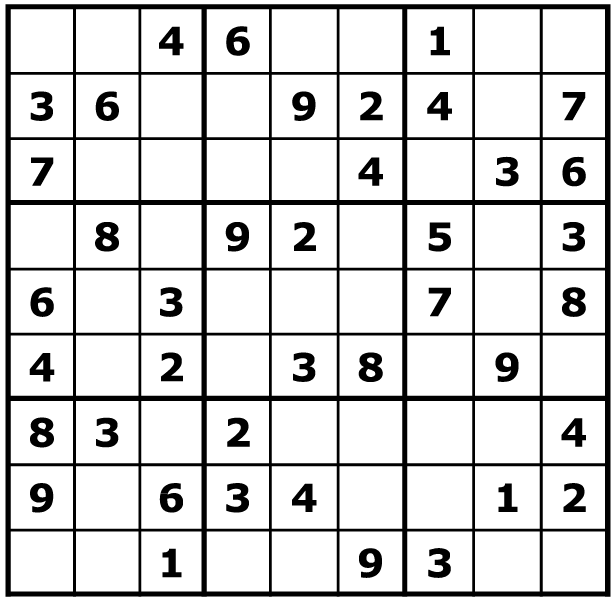
\includegraphics[scale=0.26]{primer_sudoku_neresen.png}
    \caption{Primer slagalice Sudoku}
    \label{fig:sudokuEmpty}
\end{figure}

\subsubsection{Pravila igre}
Pravila igre su vrlo jednostavna, iako rešenje često nije. Slagalicu čini kvadrat. Broj polja je najčešće 81 ($9\times9$), koji je podeljen na manje kvadrate (podkvadrate) dimenzija $3\times3$ polja. Kao početni „tragovi“, u nekoliko polja su unešene cifre, a cilj igre je da se ostala prazna polja popune tako da na kraju svaki red, kolona i podkvadrat sadrze cifre od 1 do 9 samo jedanput.\\ Sudoku slagalice su u zavisnosti od težine uglavnom podeljene na \textbf{„lake“}, \textbf{„srednje“} i \textbf{„teške“} . Treba naglasiti da težinu slagalice ne određuje samo broj unapred datih cifara, već i njihov razmeštaj u kvadratu.\\
Sudoku slagalica po pravilu ima samo \textbf{jedno moguće rešenje} (može ih imati više u slučaju da je na početku otkriven mali broj polja). U međuvremenu su se pojavile i slagalice sa $16\times16$ polja kao i druge još komplikovanije varijante, na primer kombinacija igara Sudoku i Kakuro nazvana “Killer Sudoku”. Postoji i Sudoku za decu, koji se sastoji od malog broja polja.

\begin{figure}[h]
    \centering
    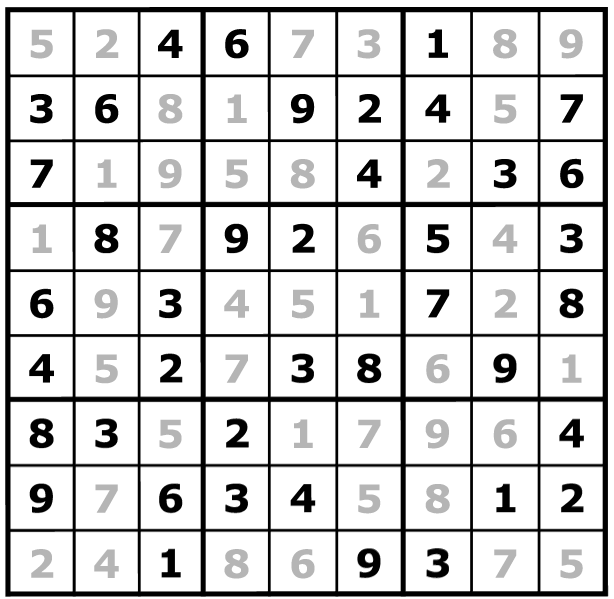
\includegraphics[scale=0.26]{primer_sudoku_resen.png}
    \caption{Rešeni primer slagalice Sudoku}
    \label{fig:sudokuFull}
\end{figure}

\subsection{Genetski algoritam}
\textbf{Genetski algoritam} je pretraživačka optimimizaciona tehnika koja teži da imitira biološku evoluciju koju su definisali Čarls Darvin i Žan-Batist Lamark. Ideja algoritma je da tretira svoje ulazne podatke problema kao hromozome.\\ Tokom vremena, populacija evoluira i prilagođava se okruženju. Bolje prilagođene jedinke imaju veću šansu da prežive i učestvuju u razmnožavanju, a time i da prenesu svoj genetski materijal u narednu generaciju. Tako slabije jedinke i njihov genetski materijal postepeno nestaju iz populacije.\\ Brojni su primeri primene genetskog algoritma, među kojima se najpre svrstava rešavanje NP-teških optimizacionih problema. Kriterijum zaustavljanja GA može biti dostignut maksimalan broj generacija, maksimalan broj generacija bez poboljšanja najbolje jedinke, isteklo unapred zadato maksimalno vreme izvršavanja algoritma, pronađeno optimalno rešenje i slično.


\subsubsection{Način izvršavanja algoritma}

Genetski algoritam polazi od inicijalne populacije jedinki, gde svaka jedinka odgovara jednom rešenju u prostoru pretrage. Potom se iterativno primenjuju genetski operatori na jedinke populacije.\\
\textbf{Prilagođenost} (engl. fitness function) jedinke se računa na osnovu funkcije cilja. Dalje, jedinke izabrane na osnovu prilagođenosti se \textbf{ukrštaju} (engl. crossover) i stvaraju nove jedinke, koje imaju karakteristike oba roditelje. Dodatno, vrši se \textbf{mutacija} (engl. mutation)nekih gena jedinki, kako bi se očuvala raznovrsnost genetskog materijala. Tako dobijene jedinke zamenjuju celu prethodnu populaciju
ili njen manje prilagođeni deo.

\subsubsection{Inicijalizacija populacije}
Populacija je podskup rešenja u  trenutnoj generaciji tj. to je skup \textbf{hromozoma}. U većini slučajeva, inicijalna populacija se generiše na slučajan način. Međutim, treba imati na umu bar bitnih stvari: važno je održavati \textbf{raznolikost populacije}, u suprtonom, može doći do prerane konvergencije kao i voditi računa o \textbf{veličini populacije}- ne bi trebalo da bude prevelika, jer to može dovesti do usporenja GA ali isto tako ne sme biti ni premala jer nam ne daje dovoljan prostor za raznoliko mešanje hromozoma. Skup \textbf{gena} (parametri u okviru rešenja) predstavlja hromozom. Geni su yzapravo odgovarajuća svostva organizma, dok se različite mogućnosti za svako svojstvo naziva genski \textbf{alel}.

\begin{figure}[h]
    \centering
    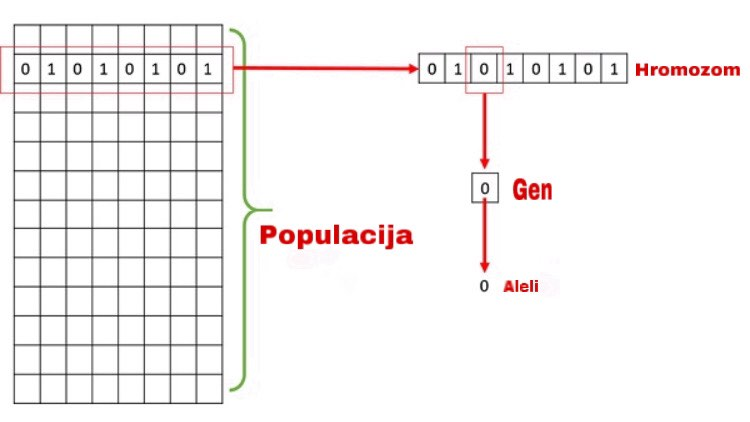
\includegraphics[scale=0.3]{oznake.jpg}
    \caption{Osnovni pojmovi GA}
    \label{fig:parts}
\end{figure}

\subsubsection{Funkcija prilagođenosti}
Funkcija prilagođenosti (eng. fitness function) nam daje ocenu kvaliteta jedinke. Prilagođenost jedinki se računa na osnovu funkcije cilja. Najčešće se za prilagođenost koristi direktno funkcija cilja, ali pod uslovom da njeno računanje nije vremenski zahtevno. U zavisnosti od konkretnog problema funkcija cilja se transformiše na različite načine. U nekim slučajevima, teško je ili gotovo nemoguće odredititi ovu vrednost. Funkcija prilagođenosti nam pomaže u odabiru pojedinaca koji će se koristiti dalje za reprodukciju.

\subsubsection{Selekcija}
Kao i u prirodi, uloga selekcije kod genetskog algoritma je odabrati jedinke koje će učestvovati u stvaranju nove populacije. Cilj je stvoriti populaciju koja je bolja od prethodne, odnosno sastoji se od jedinki koje imaju bolju fitness funkciju. Zbog toga, genetski materijal za stvaranje nove generacije mora biti kvalitetan i zato se veća verovatnoća pridružuje jedinkama sa boljom prilagođenošću. Međutim, ne treba u potpunosti zanemariti ni one sa lošijom vrednošću, jer svakako postoji verovatnoća da i one mogu učestvovati u stvaranju deteta sa dobrom prilagođenošću. Iako je pretpostavka da će kvalitetni geni sa velikom verovatnoćom preći u narednu generaciju, to ne mora uvek biti slučaj.\\
Postoji više tipova operatora selekcije.\\
Kod \textbf{rulet selekcije} (engl. roulette wheel selection), verovatnoća izbora neke jedinke je proporcionalna njenoj prilagođenosti. Nedostatak ovakve selekcije jeste mogućnost čestog izbora visoko prilagođenih jedinki, što može dovesti do preuranjene konvergencije.\\
\textbf{Turnirska selekcija}(engl. tournament selection) predstavlja alternativu rulet selekciji. To je popularna tehnika, gde se populacije dele na grupe od po k jedinki(broj k je manji od ukupne veličine populacije) koje se takmiče za prelazak u narednu generaciju, odigravajući turnire. Turnirska selekcija se takođe naziva i eliminacijska selekcija, upravo zbog svog načina rada.

\subsubsection{Ukrštanje}
Kao što smo naveli, selekcijom izabrane jedinke ulaze u proces reprodukcije, gde se primenom operatora ukrštanja i/ili mutacije proizvodi potomstvo. Ukrštanjem se kombinuju roditeljski hromozomi a rešenje se optimizuje samo u okviru postojeće oblasti. Dakle, to je proces kojim se kombinovanjem proizvoljno izabranog genetskog materijala dva ili više roditelja formira jedna ili više jedinki neposrednog potomstva tj. dece. Jedinke roditelja izabrane selekcijom ne moraju nužno da se ukrštaju. Svaki od parova hromozoma se ukršta sa nekom verovatnoćom pc. Verovatnoća (stopa) ukrštanja je uglavnom velika, uzima vrednosti iz intervala [0.6, 0.9]. Prilikom selekcije roditelja za ukrštanje potrebno je obezbediti da jedna ista jedinka ne bude odabrana za oba roditelja (u tom slučaju je generisani potomak kopija roditelja) i da ista jedinka ne učestvuje u više od jednog procesa ukrštanja ukoliko se koriste fitnes-proporcionalne sheme selekcije.\\ Postoje 3 glavne vrste ukrštanja:
\begin{enumerate}
                \item \textbf{Jednopoziciono ukrštanje:} Tačka na hromozomima oba roditelja bira se nasumično i označava se kao tzv. crossover tačka. Bitovi desno od te tačke razmenjuju se između dva matična hromozoma. 
                \item \textbf{Dvopoziciono ukrštanje:}Dve tačke ukrštanja izabrane su nasumično iz roditeljskih hromozoma. Bitovi između dve tačke se menjaju između roditelja
                \item \textbf{Uniformno ukrštanje:} U uniformnom ukrštanju, obično se svaki bit bira između bilo kog roditelja s jednakom verovatnoćom. 
\end{enumerate}

\subsubsection{Mutacija}
Mutacija je takođe operator reprodukcije čijim delovanjem se vrši izmena slučajno odabranih gena jedinke. Kako deluje nad samo jednom jedinkom, mutacija je unarni operator koji kao rezultat daje izmenjenu jedinku. Ovaj operator omogućava vraćanje korisnog genetskog materijala koji je izgubljen u selekciji i ukrštanju. Može se reći i da mutacija predstavlja odličan mehanizam za izbegavanje lokalnih ekstremuma pretragom okoline rešenja, zbog činjenice da proširuje prostor pretrage koji se razmatra uvođenjem nove genetske informacije. Time se povećava šansa za nalaženje globalnog ekstremuma.  Tačnije, ako bi cela populacija završila u nekom od lokalnih ekstermuma, jedino se slučajnom pretragom okoline rešenja pronalazi bolje, te je dovoljno da jedna jedinka nastala mutacijom bude bolja, pa da se cela populacija u nekoliko narednih generacija “preseli“ u okolinu boljeg rešenja. Parametar koji određuje verovatnoću mutacije m p jednog gena predstavlja nivo mutacije i zadaje se na početku izvršavanja genetskog algoritma. Ako nivo mutacije teži jedinici, algoritam se pretvara u algoritam slučajne pretrage rešenja, a ako teži nuli, može se očekivati zaustavljanje procesa već na samom početku procesa optimizacije u nekom lokalnom ekstremumu. Kod genetskih algoritama, mutacija se obično primenjuje sa niskom verovatnoćom, od 0.001 do 0.01, kako se ne bi narušio genetski materijal jedinki sa dobrom funkcijom prilagodjenosti.


\subsection{Brute-force}
U računarstvu jedna od poznatijih algoritamskih strategija je \textbf{brute-force}(gruba sila) ili iscrpljujuća pretraga (takođe poznata i kao generiši i testiraj), je opšta tehnika rešavanja problema koja se sastoji od sistematičnog nabrajanja svih mogućih kandidata za rešavanje i provere da li svaki kandidat zadovoljava problem. Dok je brute-force pretraga jednostavna za primenu i uvek će pronaći rešenje ako postoji, njegova cena srazmerna je broju kandidata rešenja – što u mnogim praktičnim problemima pretenduje veoma brzim rastom kako se veličina problema povećava. Dakle, brute-force pretraga se obično koristi kada je veličina problema ograničena, ili kada postoji specifičan problem heuristike koji može biti iskorišćen da se smanji skup kandidata rešenja do veličine pogodne za rukovanje. Metoda se takođe koristi kada je jednostavnost implementacije važnija od brzine.

\section{Opis rešenja zadatog problema}
U ovom poglavlju, opisaćemo način na koji smo implementirali algoritme za rešavanje Sudoku. Prvo rešenje implementirano je primenom \textbf{GA}, gde ćemo opisati sve njegove faze: funkciju cilja koju smo koristili, odabir selekcije, ukrštanje, mutaciju, kriterijum zaustavljanja kao i nešto više reći o svakoj primenjenoj metodi. Drugo rešenje implementirano je \textbf{brute-force} metodom, o kojoj će takođe biti reči u ovom poglavlju.

\subsection{Implementacija rešenja Genetskim Algoritmom}
\subsubsection{Generisanje inicijalne populacije}
Inicijalna populacija se generiše slučajno i sadrži $N_c$ jedinki. Prateći pravila za popunjavanja kolona, vrsta i 3x3 blokova koje Sudoku nalaže, polja početne populacije se popunjavaju, vrši se tzv. sejanje već korišćenih (poznatih) hromozoma. Ažurira se prilagođenost(engl. fitness function) svake jedinke i populacija se sortira na osnovu te vrednosti.
\subsubsection{Funkcija prilagodjenosti}
\subsubsection{Selekcija}
Implementiran je operator \textbf{turnirske selekcije}. Iz populacije se na slučajan način biraju 2 jedinke, zatim se od izabranih se uzima najbolja u smislu vrednosti funkcije prilagođenosti. Za parametar ‘selection rate’ koristili smo vrednost 0.85, čime smo obezbedili da bolje prilagodjena jedinka ima verovatnoću da pobedi 0.85, dok manje prilagodjena ima 0.15.
Pobednik turnira prolazi dalje i učestvuje u stvaranju naredne populacije jedinki. 
\subsubsection{Ukrštanje}
Ukrštanje se odvija kombinovanjem dvopozicionog i cikličnog ukrštanja. Najpre, na slučajan način se biraju dve tačke ukrštanja, pri čemu ukrštanje mora da sadrži najmanje jedan red a najviše osam.
Prva jedinka potomak uzima deo koda rešenja prvog roditelja do tačke ukrštanja i nakon tačke ukrštanja. Analogno, druga jedinka potomak uzima na isti način deo koda drugog roditelja. Zbog činjenice da su kolone, vrste i blokovi slagalice Sudoku permutacije, koristimo ciklično ukrštanje. Primenjujemo ga na deo ograđen tačkama ukrštanja i u njemu učestvuju delovi između tačaka ukrštanja oba roditelja.
\subsubsection{Mutacija}
Do mutacije nekog gena dolazi sa verovatnoćom mutation\_rate. Kod našeg problema pogodno je bilo koristiti tzv. \textbf{swap mutation}, odnosno mutaciju zasnovanu na zameni, jer se ona obično koristi u kodiranjima baziranim na permutaciji. Kod swap mutacije izaberemo nasumično dva gena na hromozomu i zamenimo im vrednosti. 

\begin{figure}[h]
    \centering
    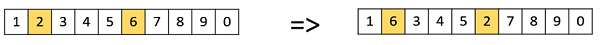
\includegraphics[scale=0.5]{swap_mutation (1).jpg}
    \caption{Mutacija zasnovana na zameni}
    \label{fig:swap}
\end{figure}
\subsubsection{Ostali aspekti algoritma}
Da se ne bi dogodilo da  pojedini potomoci budu lošiji od roditelja ili da najbolja jedinka ne pređe u narednu generaciju koristimo \textbf{princip elitizma} i uzimamo 5\% najboljih jediniki koje sigurno idu u sledeću populaciju. $N_e$ najboljih jedinki se prenosi u narednu generaciju bez promena Za ostale jedinke se primenjuje gore opisana turnirska selekcija.
\subsection{Implementacija rešenja Brute-force metodom}
Implementiran je algoritam koji rešava isti problem, problem igre Sudoku, primenom metode \textbf{brute-force}. Koristeći pravila za sudoku smanjujemo broj kandidata za rešenje i time ubrzavamo rad brute-force algoritma. Zbog toga, brojeve koji se već nalaze u nekoj vrsti, koloni ili 3x3 kvadratu ne razmatramo kao rešenje. Na pocetku popunjavamo sva ocigledna resenja, odnosno u svako polje u koje se može postaviti samo jedna vrednost, tu vrednost i postavljamo. Kada imamo vise mogućih vrednosti za jedno polje onda uzimamo jednu od vrednosti i rekurzivno pozivamo funkciju resi(), ako dođe do kontradikcije koristimo backtracking i idemo unazad i uzimamo neku drugu vrednost i opet radimo sve isto dok ne dođemo do konačnog rešenja.

\section{Eksperimentalni rezultati}

\subsection{Eksperimentalno okruženje}
Rezultati dobijeni korišćenjem gore opisanih implementiranih algoritama testirani su u sledećem okruženju:\\ 
Računar: Intel® Core™ i5 Dual Core Processor 4300M \\
Ram: 8 GB \\
Operativni sistem: Windows 10 \\

\subsection{Korišćeni parametri}
Podsetimo se najpre parametara i činjenica koje koristimo u algoritmu. Dakle, u skladu sa pravilima Sudoku, imamo da je dužina hromozoma GA niz celobrojnih vrednosti kojih ima 81, podeljenih u 9 blokova od po 9 brojeva. Takodje, imamo 9 kolona i 9 vrsti od po 9 brojeva. 
Veličina populacije je 100, a elitizma 5. Verovatnoća mutacije je 0.06. Odrađen je eksperiment nalik eksperimentu iz \href{https://seco.cs.aalto.fi/publications/2006/hyvonen-et-al-developments-in-artificial-intelligence-and-the-semantic-web-step-2006.pdf#page=91}{rada} kojim su i napravljena poređenja.
 




\section{Zaključak}




\addcontentsline{toc}{section}{Literatura}
\appendix
\bibliography{bibliografija.bib} 
\bibliographystyle{plain}


\end{document}
